\section{Design and Requirements}
\label{sec:design}

The Marketplace provides a database of available appliances, allowing
users to find appliances of interest and administrators to validate
those appliances.  To make the database easily accessible it is
implemented as a web service permitting both programmatic and
browser-based access.  The design and implementation are agnostic with
respect to the cloud distribution, allowing any cloud distribution to
interface to the Marketplace\@.

\subsection{Timeline}

A core concept within the Marketplace is the appliance timeline, a
complete history of all endorsements related to a given appliance.  An
appliance can be endorsed by more than one person to allow for third
party validation and approval of appliances.  Moreover, a particular
endorser may change her endorsement over time, updating the metadata
data associated with the appliance or explicitly deprecating the
appliance.  Endorsements are also time-limited, containing an explicit
validity period.

Users of the Marketplace can retrieve the full history, for example to
conduct an audit on why a particular appliance was authorized at a
particular point in time.  Normally however, the Marketplace users
only want to see the current endorsements for an appliance, that is
the list of the latest, non-expired endorsements from all of the
endorsers of an appliance.  This allows users and administrators alike
to decide if an appliance is currently valid.

\begin{figure}
\begin{center}
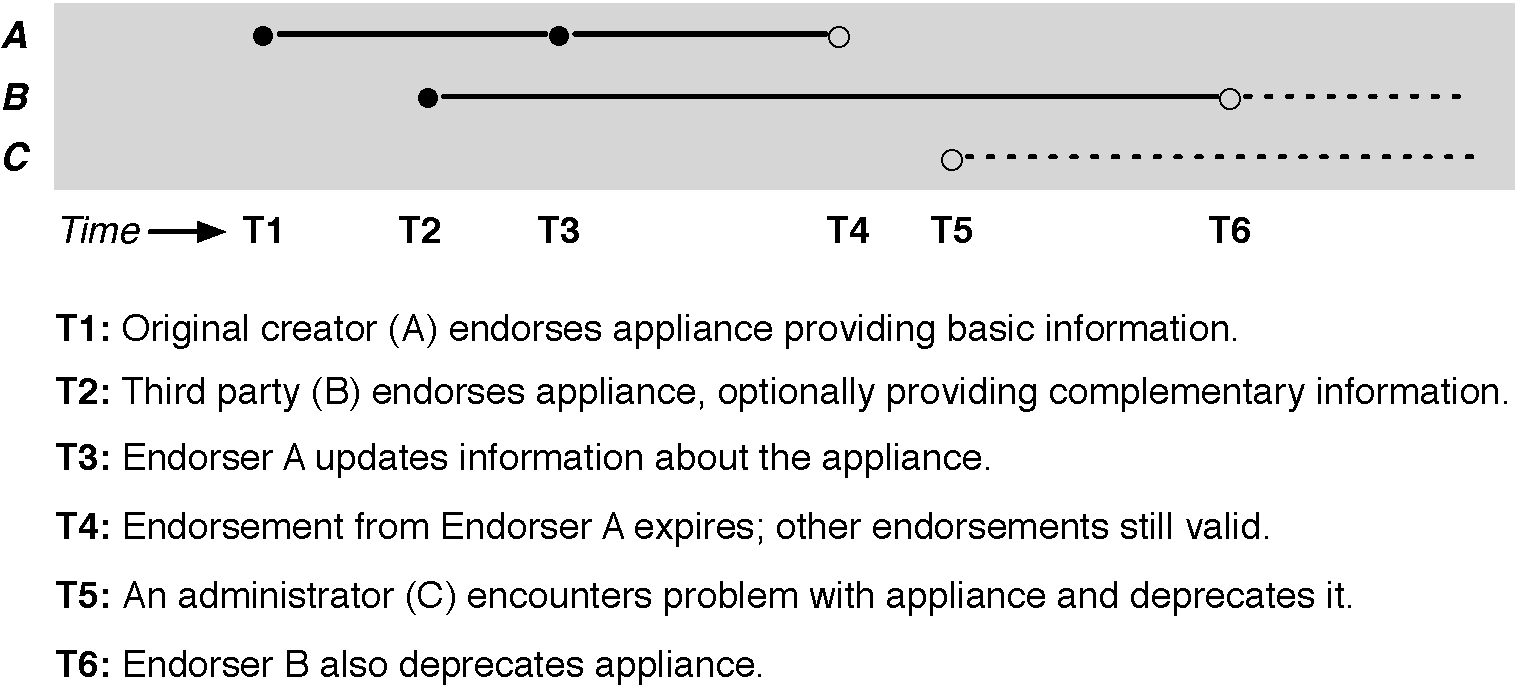
\includegraphics[width=\columnwidth]{timeline.pdf}
\end{center}
\caption{Timeline for an appliance.  The dots represent the metadata
  entries created by endorsers A, B, and C\@.}
\label{fig-timeline}
\end{figure}

\subsection{Separation of Metadata and Appliance Contents}

A conscious design decision was made to separate the storage and
transport of appliance contents from the Marketplace implementation.
Storing the appliance contents outside of the Marketplace makes it
easier to:
\begin{itemize}
\item Scale the Marketplace implementation,
\item Create mirrors of the Marketplace,
\item Ensure the implementation is independent of the transport
  protocol
\item Allow owners of the image to control access to the appliance
  contents, and
\item Relieve the Marketplace operator of the Marketplace from
  copyright and licensing concerns.
\end{itemize}
It also allows the StratusLab distribution to take advantage of
standard web servers or other cloud storage services for the appliance
contents.

\subsection{Requirements}

Table~\ref{tab:requirements} contains a detailed list of requirements
for the Marketplace as an appliance registry and for the appliance
metadata.  The core requirements have been derived from the primary
use cases and feedback from the StratusLab users and administrators.

\begin{table}
\caption{Requirements}
\label{tab:requirements}
\begin{center}
\begin{tabular}{p{0.95\columnwidth}}
\hline\hline

\\ Allow anyone to upload valid metadata descriptions to the site.

\\ Valid descriptions must be cryptographically signed.  The endorser
information must match the information in the certificate itself.

\\ Users can ``replace'' existing metadata descriptions by
  uploading a new signed description.  Nonetheless, all validated
  descriptions uploaded to the site must always be available to
  provide a timeline of the metadata evolution.

\\ Users must be able to search the metadata database on a
  reasonable subset of the possible keys.  Two required keys are the
  image identifier and the endorser's email address.

\\ Users must be able to download the original signed metadata in
  the RDF/XML format from the registry for verification.

\\ The registry should allow the metadata to be downloaded in
  alternate formats, notably JSON and HTML.

\\ The service must be easy to use from all programming languages
  (including scripting languages) and usable from a web browser.


\\
  Descriptions of available images should contain at least one
  location from which the image can be obtained.  Descriptions without
  a location are appropriate only if the image becomes unavailable.

\\ Valid descriptions must contain a valid email address.  The
  service must confirm the email address for every upload of metadata.

\\ All valid descriptions must contain a creation date for the
  endorsement.  The server must only accept descriptions with a
  creation date more recent that the current latest.

\\ There may be several sets of metadata associated with a
  particular machine or disk image. This allows third parties to
  endorse images.

\\ The underlying schema for the metadata descriptions must be
  flexible and extensible, to account for different and evolving
  needs.

\\
\hline\hline
\end{tabular}
\end{center}
\end{table}
